\subsection{双重对偶}

设 E 是左 A-模。E 的对偶 E* 的对偶 E** 称为 E 的双重对偶；它也是一个左 A-模（第3号）。对所有 \(x \in \mathbf{E}\) ，由第3号公式(10)和(12)可知，映射 \(x^* \mapsto \langle x, x^* \rangle\) 是右A-模E*上的线性形式，换言之，即双重对偶E**中的一个元素，我们将其记为 \(\tilde{x}\) ；此外，由（9）和（11）（第3号）立即得出，映射 \(c_{\mathbf{E}}: x \mapsto \tilde{x}\) （从 E 到 E**）是线性的；这个映射称为典范映射；一般来说，它既不是单射也不是满射，即使当 E 是有限生成的也是如此（参见习题9(e)及§7，第5号，定理6）。

一个 A-模 E 被称为自反的，如果典范同态 \(c_{E}:E \rightarrow E^{**}\) 是双射。

设 F 是第二个左 A-模；对于每个线性映射 \(u: E \to F\) ，映射 \(t(tu): E^{**} \to F^{**}\) （它也将记作 \({}^{tt}u\) ）是线性的，且图表

\begin{enumerate}
\def\labelenumi{(\arabic{enumi})}
\setcounter{enumi}{26}
\tightlist
\item
\end{enumerate}

\pandocbounded{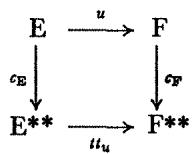
\includegraphics[keepaspectratio]{images/part002_cca49df6.jpg}}

是可交换的，这直接从定义和给出线性映射转置的公式(15)得出。

命题13. 若E是自由模（相应地，具有有限基的自由模），则典范映射 \(c_{E}:E \rightarrow E^{**}\) 是单射（相应地，双射）。

设 \((e_t)_{t \in \mathbb{T}}\) 是 \(\mathbf{E}\) 的一组基，并设 \((e_t^*)\) 为相应的坐标形式的族；根据定义，如果 \(x \in \mathbf{E}\) 满足 \(\tilde{x} = 0\) ，则 \(\langle x, e_t^* \rangle = 0\) 对所有 \(t \in \mathbb{T}\) 成立，换言之，即 \(x\) 的所有坐标均为零，因此 \(x = 0\) 。进一步假设 \(\mathbf{T}\) 是有限的；由于 \(\langle \tilde{e}_t, e_{t'}^* \rangle = \delta_{tt'}\) ， \((\tilde{e}_t)\) 是 \((e_t^*)\) 在 \(\mathbf{E}^{**}\) 中的对偶基，并且，由于 \(c_{\mathbf{E}}\) 把 \(\mathbf{E}\) 的一个基变换为 \(\mathbf{E}^{**}\) 的一个基， \(c_{\mathbf{E}}\) 是双射（§ 1，第 11 号，命题 17 的推论 3）。我们还证明了：

推论1. 设E是具有有限基的自由A-模；对于E的每个基 \((e_t)\) ， \((c_{\mathbf{E}}(e_t))\) 是 \((e_t^*)\) （E*的、与 \((e_t)\) 对偶的基）的对偶基。

在这种情况下，称 \((e_t)\) 和 \((e_t^*)\) 是彼此的对偶基。

推论2. 若E是具有有限基的自由A-模，则 \(\mathbf{E}^*\) 的每个有限基都是 \(\mathbf{E}\) 的某个基的对偶基。

只需考虑E**中给定基的对偶基，并将E典范地等同于E**即可。

推论3. 设E、F为两个均具有有限基的A-模，E（相应地，F）被典范地等同于其双重对偶E**（相应地，F**）。则对每个线性映射 \(u: \mathbf{E} \to \mathbf{F}\) ， \(^{tt}u = u\) 。

这直接从图表(27)的交换性得出。

推论4. 若P是投射模（相应地，有限生成投射模），则典范映射 \(c_{\mathbf{P}}: \mathbf{P} \to \mathbf{P}^{**}\) 是单射（相应地，双射）。

我们使用以下引理：

引理1. 设M、N是A-模E中的两个互补子模，i: M → E，j: N → E为典范单射。则图表

\begin{enumerate}
\def\labelenumi{(\arabic{enumi})}
\setcounter{enumi}{27}
\tightlist
\item
\end{enumerate}

\pandocbounded{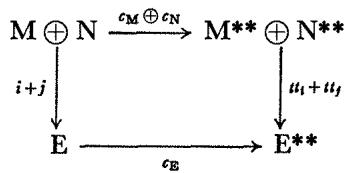
\includegraphics[keepaspectratio]{images/part002_690a791a.jpg}}

是交换的。

根据定义，对于 \(x \in \mathbf{M}\) , \(y \in \mathbf{N}\) , \(z^{*} \in \mathbf{E}^{*}\) ,

\[
\begin{array}{r l} \langle c _ {\mathrm{E}} (i (x) + j (y)), z ^ {*} \rangle & = \langle i (x) + j (y), z ^ {*} \rangle \\ & = \langle i (x), z ^ {*} \rangle + \langle j (y), z ^ {*} \rangle \\ & = \langle x, ^ {t} i (z ^ {*}) \rangle + \langle y, ^ {t} j (z ^ {*}) \rangle \\ & = \langle c _ {\mathrm{M}} (x), ^ {t} i (z ^ {*}) \rangle + \langle c _ {\mathrm{N}} (y), ^ {t} j (z ^ {*}) \rangle \\ & = \langle^ {t t} i (c _ {\mathrm{M}} (x)) + ^ {t t} j (c _ {\mathrm{N}} (y)), z ^ {*} \rangle . \end{array}
\]

既然如此，若E是自由模（相应地，具有有限基的自由模）， \(c_{E}\) 是单射（相应地，双射）；另一方面，由第6号、命题10可知， \(^{tt}i \oplus ^{tt}j\) 是双射的；图表(28)的交换性因此蕴含 \(c_{M} \oplus c_{N}\) 是单射（相应地，双射），因此 \(c_{M}\) 和 \(c_{N}\) （§1，第6号，命题7的推论1）亦然；考虑到第2号命题4，即得出推论。

